%%% Uncomment the following for normal slide show
\documentclass[10pt,serif,professionalfont]{beamer}

%%% or uncomment this for handouts
% \documentclass[handout,ignorenonframetext]{beamer}

%%% or uncomment this for the article version
% \documentclass[11pt]{article}
% \usepackage{beamerarticle}

%%% Based on a TeXnicCenter-Template by Tino Weinkauf.
%%%%%%%%%%%%%%%%%%%%%%%%%%%%%%%%%%%%%%%%%%%%%%%%%%%%%%%%%%%%%

%\usepackage[utf8]{inputenc}
\usepackage[ansinew]{inputenc}

\usepackage[english]{babel}
%\usepackage[bibnewpage]{apacite}
%\usepackage{natbib}

\usepackage{fancyhdr}
\usepackage{setspace}
\usepackage{indentfirst}
\usepackage{booktabs}

\usepackage{amsmath, amsbsy, amssymb}

\usepackage{graphics}
\usepackage{graphicx}
\usepackage{subfig}
\usepackage{caption}
\usepackage{float}
\usepackage{rotating}
\usepackage{pdflscape}
\usepackage{caption}

\usepackage{soul} %for highlighting for mark?
\usepackage{color}
%\sethlcolor{white}




%%%%%%%%%%%%%%%%%%%%%%%%%%%%
%%% Beamer Stuff
%%%%%%%%%%%%%%%%%%%%%%%%%%%%

\let\Tiny=\tiny

\mode<article>
{
  \usepackage{fullpage}
  \usepackage{pgf}
  \usepackage{hyperref}
  \setjobnamebeamerversion{example.beamer}
}

\mode<presentation>
{
  % \usetheme{Dresden}
  % \usetheme{Marburg}
  % \usetheme{Hannover}
  \usetheme{Singapore}
  % \useoutertheme{smoothbars}
  % \useoutertheme{infolines}
  \usecolortheme{seagull}
  \setbeamercovered{invisible}
  \setbeamertemplate{navigation symbols}{}%remove navigation symbols
%  \setbeamertemplate{footline}[page number]
  \setbeamertemplate{footline}[frame number]
}

\mode<handout>
{
%%% In handout mode give the individual pages a light grey background
\setbeamercolor{background canvas}{bg=black!5}
%%% Put more than one frame on each page to save paper.
\usepackage{pgfpages}
\pgfpagesuselayout{4 on 1}[letterpaper,border shrink=3mm, landscape]
% \pgfpagesuselayout{2 on 1}[letterpaper,border shrink=5mm, portrait]
% \setbeameroption{show notes}
}
% \usepackage[latin1]{inputenc}

\setbeamertemplate{itemize items}[default]
\setbeamertemplate{enumerate items}[default]
\setbeamertemplate{frametitle continuation}[from second]

\setbeamercovered{transparent}

%\usepackage{appendixnumberbeamer}

\usepackage[T1]{fontenc}
\usepackage[osf]{mathpazo}
%\linespread{1.05}         % Palatino needs more leading (space between lines)

%\usepackage{pxfonts}
%\usepackage{eulervm}

 %David I didn't have access to this file!!!
%% Based on a TeXnicCenter-Template by Tino Weinkauf.
%%%%%%%%%%%%%%%%%%%%%%%%%%%%%%%%%%%%%%%%%%%%%%%%%%%%%%%%%%%%%

%\usepackage[utf8]{inputenc}
\usepackage[ansinew]{inputenc}

\usepackage[english]{babel}
%\usepackage[bibnewpage]{apacite}
%\usepackage{natbib}

\usepackage{fancyhdr}
\usepackage{setspace}
\usepackage{indentfirst}
\usepackage{booktabs}

\usepackage{amsmath, amsbsy, amssymb}

\usepackage{graphics}
\usepackage{graphicx}
\usepackage{subfig}
\usepackage{caption}
\usepackage{float}
\usepackage{rotating}
\usepackage{pdflscape}
\usepackage{caption}

\usepackage{soul} %for highlighting for mark?
\usepackage{color}
%\sethlcolor{white}




%%%%%%%%%%%%%%%%%%%%%%%%%%%%
%%% Beamer Stuff
%%%%%%%%%%%%%%%%%%%%%%%%%%%%

\let\Tiny=\tiny

\mode<article>
{
  \usepackage{fullpage}
  \usepackage{pgf}
  \usepackage{hyperref}
  \setjobnamebeamerversion{example.beamer}
}

\mode<presentation>
{
  % \usetheme{Dresden}
  % \usetheme{Marburg}
  % \usetheme{Hannover}
  \usetheme{Singapore}
  % \useoutertheme{smoothbars}
  % \useoutertheme{infolines}
  \usecolortheme{seagull}
  \setbeamercovered{invisible}
  \setbeamertemplate{navigation symbols}{}%remove navigation symbols
%  \setbeamertemplate{footline}[page number]
  \setbeamertemplate{footline}[frame number]
}

\mode<handout>
{
%%% In handout mode give the individual pages a light grey background
\setbeamercolor{background canvas}{bg=black!5}
%%% Put more than one frame on each page to save paper.
\usepackage{pgfpages}
\pgfpagesuselayout{4 on 1}[letterpaper,border shrink=3mm, landscape]
% \pgfpagesuselayout{2 on 1}[letterpaper,border shrink=5mm, portrait]
% \setbeameroption{show notes}
}
% \usepackage[latin1]{inputenc}

\setbeamertemplate{itemize items}[default]
\setbeamertemplate{enumerate items}[default]
\setbeamertemplate{frametitle continuation}[from second]

\setbeamercovered{transparent}

%\usepackage{appendixnumberbeamer}

\usepackage[T1]{fontenc}
\usepackage[osf]{mathpazo}
%\linespread{1.05}         % Palatino needs more leading (space between lines)

%\usepackage{pxfonts}
%\usepackage{eulervm}


\usepackage{outlines}

\title{Applying the Axioms of Additive Conjoint Measurement to a Hierarchy of Latent Variable Models}

\author{Benjamin Domingue\inst{1} \and David Torres Irribarra\inst{2} \and Ronli Diakow\inst{3}}

\subject{Tenable Assessment}

\date{International Meeting of the Psychometric Society \\ July 25, 2013}

\institute[University of California, Berkeley]{
  \inst{1} University of Colorado at Boulder \and
  \inst{2} University of California, Berkeley \and
  \inst{3} New York University}

\begin{document}

\frame{\maketitle}

\section{Two methods}
\begin{frame}
    \frametitle{Score scales and latent structure}

    different models, score scales, inferences, individual differences

\end{frame}

\begin{frame}
    \frametitle{A tale of two methods}

    Torres Irribarra and Diakow -- framework / hierarchy of latent variable models according to latent structure / implied/supportable scale (qualitative, ordinal, interval), check using standard model fit indices

    Domingue -- do data possess sufficient structure, as judged by the axioms of conjoint measurement, to yield interval scales%bd whether data consistent with the Rasch model possessed sufficient structure, according to the axioms of Additive Conjoint Measurement (ACM; Luce \& Tukey, 1964), to support a score scale with interval properties

\end{frame}

\begin{frame}
    \frametitle{A hierarchy of latent variable models}

    [equations]

    [figures]

\end{frame}

\begin{frame}
    \frametitle{Additive conjoint measurement (\textsc{acm})}

    If the axioms of \textsc{acm} hold in item response data, then it is possible to create interval scales for the abilities/difficulties of the people/items that generated the data. %bd is [unclear to me]

    axioms: Focus is on single and double cancellation axioms. %bdcancellation, solvability, archimedes

\end{frame}

\begin{frame} %bd
    \frametitle{Cancellation axioms}
    Single cancellation: Rows or columns can be consistently ordered.%bd
    %bd [set of matrices used to explain]

Easiest to see in a $3 \times 3$ matrix formed by the selection of 3 items and 3 abilities:
\[
\begin{array}{ccc}
  \cdot&x_{12} &x_{13}  \\
  x_{21}&\cdot&x_{23} \\
  x_{31} & x_{32}&\cdot\\
\end{array}.
\]
Two forms:
\begin{enumerate}
\item If $x_{21}<x_{12} \& x_{32}<x_{23} \text{then} x_{31}<x_{13}$.
\item If $x_{21}>x_{12} \& x_{32}>x_{23} \text{then} x_{31}>x_{13}$.
\end{enumerate}
Key is that double cancellation imposes some order on the very messy minor diagonal.

\end{frame}

\begin{frame}
    \frametitle{Applying the axioms of \textsc{acm}}

    Domingue method to check cancellation axioms -- estimate posterior for a cell using relevant cancellation constraints to form the jumping distribution and then check if observed proportions fit within posterior%bdDomingue method to check cancellation axioms -- estimate credible intervals with relevant cancellation constraints and check if observed data within interval

    Previously applied to Rasch model

\end{frame}

\begin{frame}
    \frametitle{}

    [new figure showing relationship of hierarchy to axioms]

\end{frame}

\begin{frame}
    \frametitle{}

\end{frame}


\section{Study design}

\begin{frame}
    \frametitle{Hypotheses/Questions} %bd}

    \begin{enumerate}
    \item \textsc{un} model -- most violations
    \item symmetry between \textsc{mon} and \textsc{iio} models?
    \item order: \textsc{mon} / \textsc{iio}, \textsc{dm}, \textsc{lcr} / \textsc{rm}
    \end{enumerate}


    If hold, straightforward criteria to distinguish latent structure

\end{frame}

\begin{frame}
    \frametitle{Simulation design}

    generate data under each of six models

    1000 people in 6 latent classes and 50 items in 6 latent groups

    50 replications for each model

\end{frame}

\begin{frame}
    \frametitle{Analysis}

    ConjointChecks, each single cancellation and double cancellation

    \% weighted violations

\end{frame}


\section{Results}

\begin{frame}
    \frametitle{Double cancellation}

    [include figure]

\end{frame}

\begin{frame}
    \frametitle{Single cancellation -- Person ordering}

    \centering 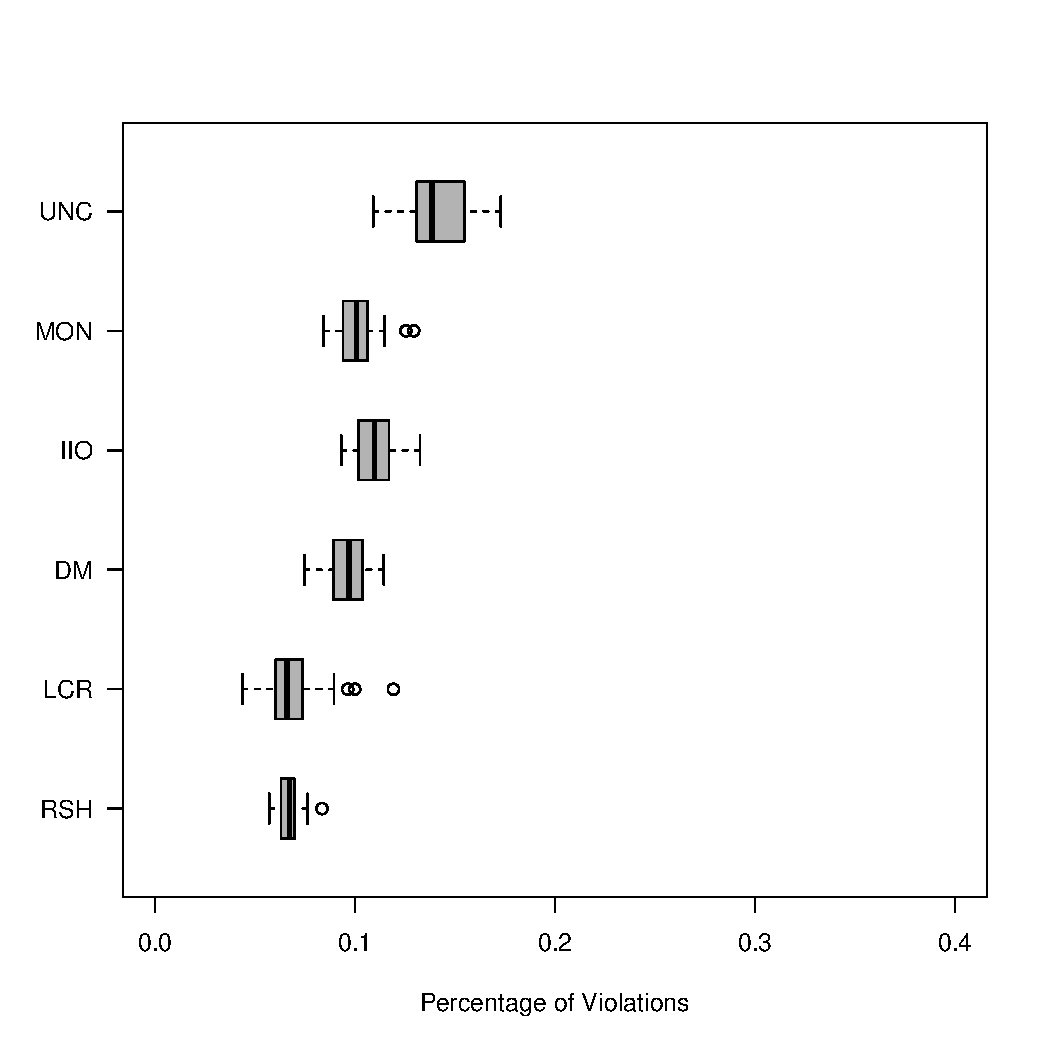
\includegraphics[width=0.75\textwidth]{./figs/violations_columns_weighted.pdf}

\end{frame}

\begin{frame}
    \frametitle{Single cancellation -- Item ordering}

    \centering 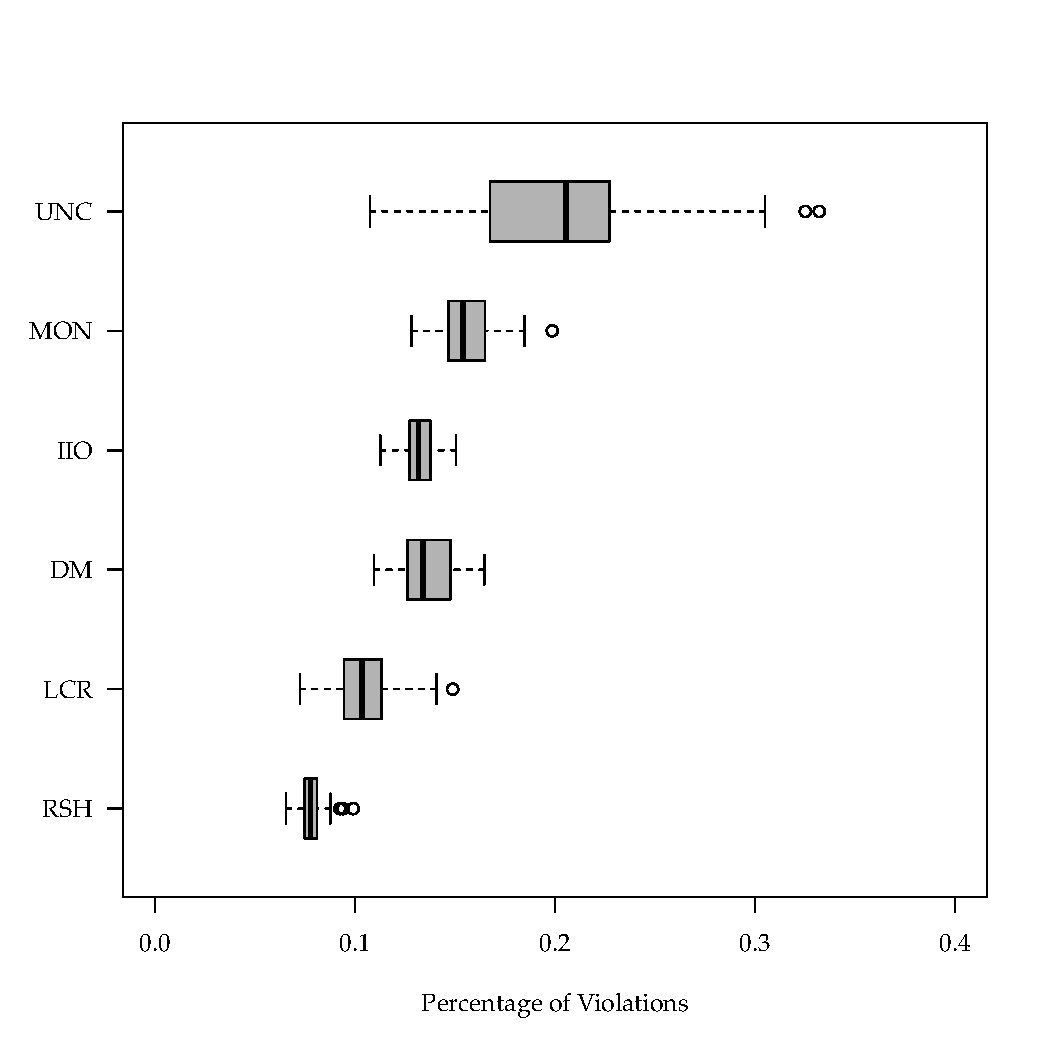
\includegraphics[width=0.75\textwidth]{./figs/violations_rows_weighted.pdf}

\end{frame}


\section{Discussion}

\begin{frame}
    \frametitle{Person monotonicity versus item ordering}

    precision / aggregation

    how this simulation is different from how we usually treat persons and items

\end{frame}

\begin{frame}
    \frametitle{Reconsidering double cancellation}

\end{frame}

\begin{frame}
    \frametitle{Further thoughts}
    
    return to the 3 hypotheses/questions

\end{frame}

\frame[contactinfo]{

    \begin{center}

    \Large Applying the Axioms of Additive Conjoint Measurement to a Hierarchy of Latent Variable Models

    \vspace{10mm}

    \small

    \begin{tabular}{rl}

    	xxx@xxx.xxx          & \textsc{Benjamin Domingue} \\
        dti@berkeley.edu     & \textsc{David Torres Irribarra} \\
    	rdiakow@berkeley.edu & \textsc{Ronli Diakow}
    	
    \end{tabular}
	
    \end{center}

    \vspace{10mm}

%    \scriptsize
%    \hspace{5mm} Torres Irribarra, D., and Diakow, R.  (2011, July).  Model Selection for Tenable Assessment: Selecting a Latent Variable Model by Testing the Assumed Latent Structure.  Paper presented at the 76th Annual and 17th International Meeting of the Psychometric Society, Hong Kong.


}


%back-up slides
\appendix

%fix so slide numbering ignores back-up slides
\newcounter{finalpage}
\setcounter{finalpage}{\value{page}}
\newcounter{finalframe}
\setcounter{finalframe}{\value{framenumber}}
\setbeamertemplate{footline}{}

\begin{frame}

    \centering Appendix Slides

\end{frame}

%fix so slide numbering ignores back-ups
\setcounter{page}{\value{finalpage}}
\setcounter{framenumber}{\value{finalframe}}

\end{document}


\begin{frame}
    \frametitle{}

\end{frame}
